\documentclass{article}
\usepackage{amsmath}
\usepackage{amssymb}
\usepackage{setspace}
\usepackage{mathrsfs}
\newenvironment{nscenter}
{\parskip=0pt\par\nopagebreak\centering}
{\par\noindent\ignorespacesafterend}
\usepackage{graphicx}
\graphicspath{ {images/} }
\begin{document}
\begin{spacing}{1.5}
\section{Four special matrices}
1. Toeplitz matrix

A Toeplitz matrix or diagonal-constant matrix, named after Otto Toeplitz, is a matrix in which each descending diagonal from left to right is constant. For instance:
\\\begin{center}
	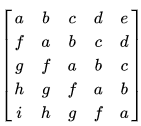
\includegraphics[width=0.2\textwidth]{Toeplitz_matrix1.png} \\ 
\end{center}
2. Circulant matrix

a circulant matrix is a special kind of Toeplitz matrix where each row vector is rotated one element to the right relative to the preceding row vector. For instance:
\\\begin{center}
	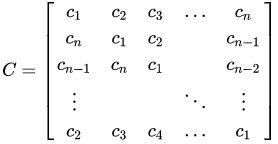
\includegraphics[width=0.35\textwidth]{circulant_matrix.png}
\end{center}

In numerical analysis, circulant matrices are important because they are diagonalized by a discrete Fourier transform, and hence linear equations that contain them may be quickly solved using a fast Fourier transform.
\\\\3. Change $T_{11}$ in Toeplitz matrix

Here we've a free variable in Toeplitz matrix $T$ at position $T_{11}$.
\\\\4. Change $T_{11}$ and $T_{nn}$ in Toeplitz matrix

Here we've two free variables in Toeplitz matrix $T$ at position $T_{11}$ and $T_{nn}$.


\section{Differential eqns and Difference eqns}
Part 1. Notation of high order derivative

For n-th derivative, the notation is $\frac{d^ny}{dx^n}$ or $\frac{d^nf(x)}{dx^n}$. Sample of meaning of this notation: $\frac{d^2y}{dx^2}=\frac{d}{dx}(\frac{dy}{dx})$.
\\\\Part 2. First order difference

To calculate first order discrete derivative(difference) of $u(x)$, we have three choices: forward, backward and centered:

\hspace*{2cm}forward $\Delta_F$: $u'(x)\approx \frac{u(x+h)-u(x)}{h}$

\hspace*{2cm}backward $\Delta_B$: $u'x)\approx \frac{u(x)-u(x-h)}{h}$

\hspace*{2cm}centered($\frac{forward - backward}{2}$) $\Delta_C$: $u'(x)\approx \frac{u(x+h)-u(x-h)}{2h}$ 

We would like use centered difference for first order difference. The reason comes from the loss of accuracy:

First, recall Taylor series:
\begin{nscenter}
$f(x) = f(a)+{\frac {f'(a)}{1!}}(x-a)+{\frac {f''(a)}{2!}}(x-a)^{2}+{\frac {f'''(a)}{3!}}(x-a)^{3}+\cdots$
\end{nscenter}

Second, from Taylor series, we have:
\begin{nscenter}
$u(x+h)=u(x)+hu'(x) + \frac{h^2}{2!}u''(x) + \frac{h^3}{3!}u'''(x) + \cdots$
$u(x-h)=u(x)-hu'(x) + \frac{h^2}{2!}u''(x) - \frac{h^3}{3!}u'''(x) + \cdots$
\end{nscenter}

Finally, inserting $u(x+h)$, $u(x-h)$ in three kind of differences, $\Delta_F = \Delta_B \approx u'(x) + o(h)$, $\Delta_C\approx u'(x) + o(h^2)$.
\\\\Part 3. Second order difference

The best way to calculate second order discrete derivative(difference) is $u''(x) \approx \frac{-u(x+h) + 2u(x) -u(x-h)}{h^2}$, or $h$ with 1 such that $u''(x) \approx -u(x+1) + 2u(x)-u(x-1)$. You may wonder where this form comes from. This form is $\Delta_F\Delta_B(=\Delta_B\Delta_F)$, which is better than $\Delta_C \Delta_C$.

Having $\Delta(\Delta u(x)) = -u(x+1) + 2u(x)-u(x-1)$, we can write multi $\Delta(\Delta u(x))$ in matrix form. Here is a funny thing to see in the matrix form

$$
\Delta = 
\begin{bmatrix}
1 & 2 & -1 \\
  & 1 & 2 & -1 \\
  &   & 1 & 2 & -1
\end{bmatrix}
\begin{bmatrix}
u(i-2) \\
u(i-1) \\
u(i) \\
u(i+1) \\
u(i+2)
\end{bmatrix}
$$

Above is the second order difference of $u(x)$ at five points with gap 1. You can insert the five point with any function $g$. If the function is a linear/quadratic function, $\Delta$ is a vector with all element being 0/a constant! You can check this. The reason behind the funny thing is that $\Delta$ is second order discrete derivative. Also note that the matrix composed of 1, 2, -1 is a Toeplitz matrix.
\\\\ Part 3. Differential equations

For example, $-\frac{d^2u}{dx^2}=1$, $\frac{du}{dx}(0)=0$, $u(1)=0$. 

This is very easy to calculate.


\section{Solving a Linear System}
Part 1. Four matrix decompositions

All these four decompositions are covered in 18.06 Linear Algebra.

Elimination: $A=LU$ and $A=LDU$

Orthogonalization: $A=QR$

Eigenvalues: $A=S\Lambda S^{-1}$

Singular values: $A=U\Sigma V^T$
\\Supplement:

For a matrix $A=BDB^T$, where $D$ is a diagonal matrix, $A$ is symmetric, since $A^T=BD^TB^T=BDB^T=A$. Then LDU decomposition on $A$, we get $A=LDL^T$.
\\\\Part 2.

More detail is needed.

For $AX=I$, we know $X=A^{-1}$. The deep insight is that columns of $A^{-1}$ are responses to $n$ impulses(columns of $I$).


\section{Delta function day}
Part 1. Definition of Delta function

The Dirac delta can be loosely thought of as a function on the real line which is zero everywhere except at the origin, where it is infinite,
\begin{nscenter}
${\displaystyle \delta (x)={\begin{cases}+\infty ,&x=0\\0,&x\neq 0\end{cases}}}$
\end{nscenter}
and which is also constrained to satisfy the identity,
\begin{nscenter}
	${\displaystyle \int _{-\infty }^{\infty }\delta (x)\,dx=1}$
\end{nscenter}
\\\\Part 2. Delta function and differential eqns

For example, 
$$
\begin{cases}
-\frac{d^2u}{dx}=\delta(x-a), where \, 0 < a < 1 \qquad (1)\\
u(0)=0 \qquad (2)\\
u(1)=0 \qquad (3)
\end{cases}$$

To get the solution of $u(x)$, first let's see what equation (1) means. (1) tells us that $u(x)$ consists two lines, and there is a turning point, because only in this way can we get (1), for instance(not the solution for (1), (2), (3):)
\\\begin{center}
	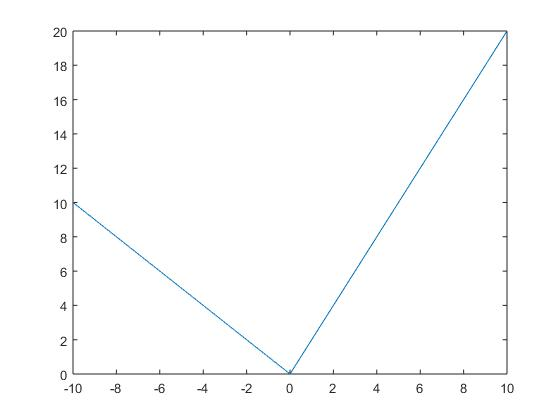
\includegraphics[width=0.4\textwidth]{piecewise_func.jpg} \\ 
\end{center}

But we have a better way to decompose the picture above as $u(x) = -R(x-a) + C + Dx$, where $R(x)$ is Ramp function. There are many equivalent definitions of Ramp function, here are two of them. 
\begin{nscenter}
	$R(x):={\begin{cases}x,&x\geq 0;\\0,&x<0\end{cases}}$ \qquad ${\displaystyle R(x):=\operatorname {max} (0, x)} $
\end{nscenter}

The convenience of $u(x) = -R(x-a) + C + Dx$ is that we can easily insert equations (2) and (3) to get $C$ and $D$.
\\\\Part 3. Boundary in differential eqns

We name equations (2) and (3) as boundaries in the differential eqns in part 2. Boundaries as $u(x)=a$ and $u'(x)=a$ are called fixed boundary and free boundary.

You can see that if we have at least one fixed boundaries, we can get only one solution. If the two boundaries are both free boundaries, we have numerous solutions.

\section{Eigenvalues(part 1)}
Covered in 18.06 Linear Algebra.

\section{Eigenvalues(part 2), positive definite(part 1)}
Covered in 18.06 Linear Algebra.

\section{Positive definite day}
Covered in 18.06 Linear Algebra.

\end{spacing}
\end{document}